\documentclass[otchet]{SCWorks}
\usepackage{preamble}

\begin{document}

\chair{информатики и программирования}
\title{Метод градиентного спуска и его модификации в задачах обучения нейронных сетей}
\course{1}
\group{111}
\napravlenie{02.03.02 "--- Фундаментальная информатика \\
	и информационные технологии}
\author{Трофимова Ильи Владимировича}

\chair{вычислительной математики и информатики}

\chtitle{доцент, к.\,ф.-м.\,н.}
\chname{С.\,В.\,Миронов}

\satitle{научный руководитель}
\saname{М.\,Чернигин}

\date{2026}

\maketitle
\secNumbering
\tableofcontents

\intro
	
	Метод градиентного спуска (Gradient Descent, GD) является фундаментальным алгоритмом оптимизации в машинном обучении, особенно в задачах обучения нейронных сетей \cite{goodfellow}. 
	В рамках данной работы рассматриваются различные модификации этого метода. 
	Переменные, участвующие в формулах, будут обозначаться моноширинным шрифтом: \texttt{$\theta$} — вектор параметров, \texttt{$\alpha$} — скорость обучения, \texttt{$J(\theta)$} — целевая функция.
	
	На рисунке~\ref{fig:neural_network} представлена архитектура многослойной нейронной сети, для обучения которой применяется метод градиентного спуска.
	
\begin{figure}[H]
	\centering
	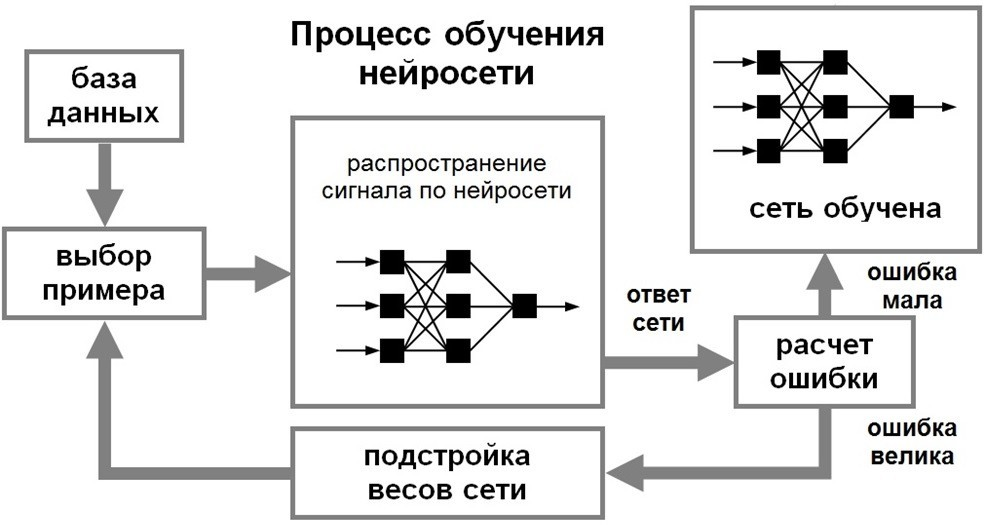
\includegraphics[width=0.8\textwidth]{images/sxema.jpeg}
	\caption{Архитектура нейронной сети с одним скрытым слоем}
	\label{fig:neural_network}
\end{figure}
	
	\section{Математическая постановка задачи}
	
	\subsection{Стандартный градиентный спуск}
	
	Классический метод градиентного спуска для минимизации функции \texttt{$J(\theta)$} определяется следующей итерационной формулой:
	
	\begin{equation}
		\label{eq:gd}
		\theta_{t+1} = \theta_t - \alpha \nabla J(\theta_t)
	\end{equation}
	
	где $\nabla J(\theta_t)$ — градиент функции потерь в точке $\theta_t$.
	
	\subsection{Стохастический градиентный спуск}
	
	В отличие от пакетного метода, SGD использует один случайный пример для оценки градиента:
	
	\begin{equation}
		\label{eq:sgd}
		\theta_{t+1} = \theta_t - \alpha \nabla J_i(\theta_t)
	\end{equation}
	
	где $i$ — индекс случайно выбранного обучающего примера \cite{bottou}.
	
	\subsection{Метод Адама (Adam)}
	
	Алгоритм Adam сочетает преимущества RMSprop и Momentum:
	
	\begin{equation}
		\label{eq:adam}
		\theta_{t+1} = \theta_t - \frac{\alpha}{\sqrt{\hat{v}_t} + \epsilon} \hat{m}_t
	\end{equation}
	
	где $m_t$ и $v_t$ — оценки первого и второго моментов градиента \cite{kingma}.
	
	\section{Экспериментальные результаты}
	
	В таблице~\ref{tab:comparison} представлено сравнение скорости сходимости различных методов оптимизации.
	
	\begin{table}[H]
		\centering
		\caption{Сравнение методов градиентного спуска}
		\label{tab:comparison}
		\begin{tabular}{|c|c|c|c|}
			\hline
			\textbf{Метод} & \textbf{Итераций до сходимости} & \textbf{Время (сек)} & \textbf{Точность} \\
			\hline
			GD & 1000 & 45.2 & 0.892 \\
			\hline
			SGD & 800 & 12.5 & 0.875 \\
			\hline
			Adam & 300 & 8.3 & 0.901 \\
			\hline
		\end{tabular}
	\end{table}
	
	На рисунке~\ref{fig:learning_curve} показаны кривые обучения для трёх методов.
	
	\begin{figure}[H]
		\centering
		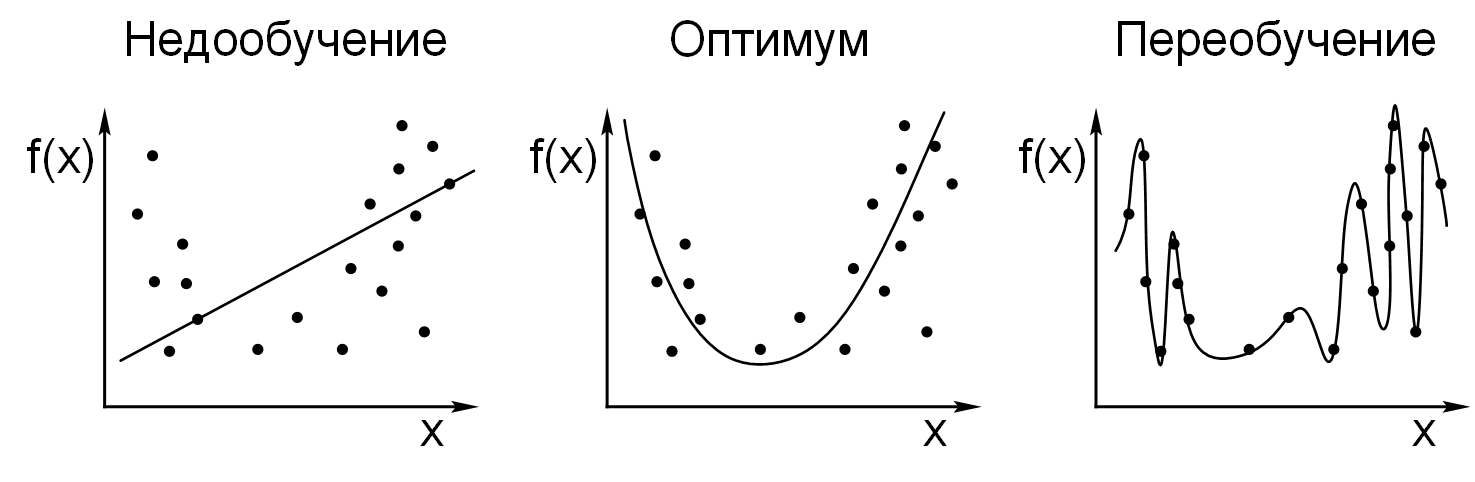
\includegraphics[width=0.8\textwidth]{images/grafik.png}
		\caption{Кривые сходимости методов оптимизации}
		\label{fig:learning_curve}
	\end{figure}
	
	\section{Реализация алгоритмов}
	
	Ниже представлена реализация метода градиентного спуска на языке \texttt{Python} с использованием библиотеки \texttt{NumPy}.
	
	\subsection{Код на Python}
	
	\inputminted{python}{code/example1.py}
	
	\subsection{Код на C++}
	
	\inputminted{cpp}{code/example2.cpp}
	
	\subsection{Пояснение к коду}
	
	В листинге~1 функция \texttt{gradient\_descent} принимает параметры:
	\begin{itemize}
		\item \texttt{X} — матрица признаков;
		\item \texttt{y} — вектор целевых значений;
		\item \texttt{alpha} — скорость обучения;
		\item \texttt{num\_iters} — количество итераций.
	\end{itemize}
	Вычисления градиента выполняются с использованием векторизации, что повышает производительность.
	
	\conclusion

В работе рассмотрены классический градиентный спуск, стохастический градиентный спуск и алгоритм Adam. Проведено сравнение методов и приведены примеры реализации на Python и C++.

\bibliographystyle{ugost2003}
\bibliography{thesis}

\end{document}
